\chapter{Background}
\label{cha:background}

In this Chapter, we define the terminology from graph theory that is relevant to and used in this thesis. \todo{Expand on introduction}

\section{Definitions}

\todo{Vertex-cut, subdivided edges}

% Graph explanation
A \textbf{graph} $G$ is a mathematical structure represented by an ordered pair $(V(G), E(G))$ consisting of a set of vertices \textbf{vertices} $V(G)$ (singular: vertex) and a (multi-)set of \textbf{edges} $E(G)$ which are unordered pairs of vertices from $V(G)$. The \textbf{order} of a graph is its number of vertices. Vertices are called \textbf{adjacent} if they share an edge. A graph is called a \textbf{simple} graph if there are no duplicate edges, and no edge exists which holds the same vertex twice. In a simple graph, the \textbf{degree} of a vertex is the number of edges that are incident on the vertex. Similarly, the minimum (maximum) degree of a graph is the minimum (maximum) degree of all its vertices. In the rest of this thesis, \emph{graph} is used to refer to simple graphs. Graphs are often represented graphically with circles representing vertices, and lines ending at circles to represent edges between two vertices, such as in Figure~\ref{fig:example-simple}\cite{book:bondy-definitions}.

A graph is called \textbf{planar} if it can be drawn in the plane such that edges do not cross other edges or vertices~\cite{book:bondy-definitions}. The graph in Figure~\ref{fig:example-simple} is planar, while that in Figure~\ref{fig:example-non-planar} is not.

\todo{Add figures relating to literature}

\begin{figure}
    \centering
    % --- Original graph ---
    \begin{subfigure}{0.25\textwidth}
    \centering
    \resizebox{\linewidth}{!}{
    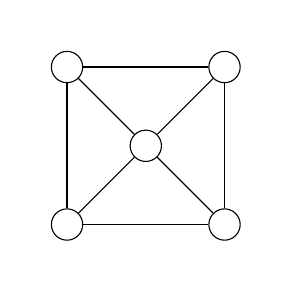
\begin{tikzpicture}[every node/.style={circle, draw, fill=white, inner sep=4pt}]
    \path[use as bounding box] (-0.5,-0.5) rectangle (2.5,2.5);
    \node (A) at (0,0)  {};
    \node (B) at (2,0)  {};
    \node (C) at (2,2)  {};
    \node (D) at (0,2)  {};
    \node (E) at (1,1)  {};

    \draw (A) -- (B) -- (C) -- (D) -- (A);
    \draw (A) -- (E);
    \draw (B) -- (E);
    \draw (C) -- (E);
    \draw (D) -- (E);
    \end{tikzpicture}
    }

    \caption{}
    \label{fig:example-simple}
    \end{subfigure}
    % --- Non-planar graph ---
    \begin{subfigure}{0.25\textwidth}
    \centering
    \resizebox{\linewidth}{!}{
    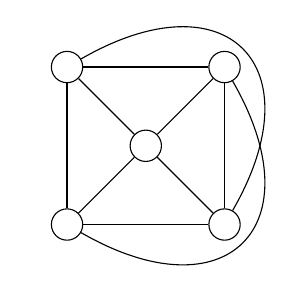
\begin{tikzpicture}[every node/.style={circle, draw, fill=white, inner sep=4pt}]
    \path[use as bounding box] (-0.5,-0.5) rectangle (2.5,2.5);
    \node (A) at (0,0)  {};
    \node (B) at (2,0)  {};
    \node (C) at (2,2)  {};
    \node (D) at (0,2)  {};
    \node (E) at (1,1)  {};

    % Only the cycle highlighted
    \draw (A) -- (B) -- (C) -- (D) -- (A);
    \draw (A) -- (E);
    \draw (B) -- (E);
    \draw (C) -- (E);
    \draw (D) -- (E);
    % Curved outer edges
    \draw[out=-30, in=-60, looseness=2] (A) to (C);
    \draw[out=60, in=30, looseness=2] (B) to (D);

    \end{tikzpicture}
    }

    \caption{}
    \label{fig:example-non-planar}
    \end{subfigure}

    % --- Longest cycle ---
    \begin{subfigure}{0.25\textwidth}
    \centering
    \resizebox{\linewidth}{!}{
    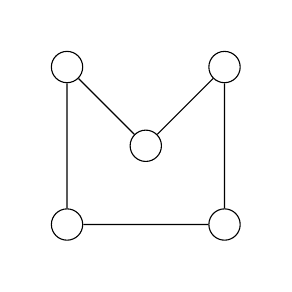
\begin{tikzpicture}[every node/.style={circle, draw, fill=white, inner sep=4pt}]
    \path[use as bounding box] (-0.5,-0.5) rectangle (2.5,2.5);
    \node (A) at (0,0)  {};
    \node (B) at (2,0)  {};
    \node (C) at (2,2)  {};
    \node (D) at (0,2)  {};
    \node (E) at (1,1)  {};

    % Only the cycle highlighted
    \draw (A) -- (B) -- (C) -- (E) -- (D) -- (A);
    \end{tikzpicture}
    }

    \caption{}
    \label{fig:example-cycle}
    \end{subfigure}
    % --- Path ---
    \begin{subfigure}{0.25\textwidth}
    \centering
    \resizebox{\linewidth}{!}{
    \begin{tikzpicture}[every node/.style={circle, draw, fill=white, inner sep=4pt}]
    \path[use as bounding box] (-0.5,-0.5) rectangle (2.5,2.5);
    \node (A) at (0,0)  {};
    \node (C) at (2,2)  {};
    \node (D) at (0,2)  {};
    \node (E) at (1,1)  {};

    % Example path
    \draw (A) -- (D) -- (E) -- (C);
    \end{tikzpicture}
    }

    \caption{}
    \label{fig:example-path}
    \end{subfigure}
    \caption{\subref*{fig:example-simple} A simple graph, \subref*{fig:example-non-planar} A simple non-planar graph \subref*{fig:example-cycle} A cycle, \subref*{fig:example-path} A path}
    \label{fig:example}
\end{figure}

% Subgraph explanation
A \textbf{subgraph} $F$ of a graph $G$ is a graph for which $V(F) \subseteq V(G)$ and $E(F) \subseteq E(G)$, and the edges $E(F)$ only contain vertices in $V(F)$. If the subgraph $F$ is the result of removing one vertex $v$ and the edges incident on $v$ from $G$ (notation: $G - v$), then we say $F$ is a vertex-deleted subgraph of $G$. Figure~\ref{fig:example-cycle} and~\ref{fig:example-path} are both subgraphs of~\ref{fig:example-simple}, and Figure~\ref{fig:example-path} is a vertex-deleted subgraph of Figure~\ref{fig:example-cycle}. Every graph in Figure~\ref{fig:example} is a subgraph of the graph in Figure~\ref{fig:example-non-planar}~\cite{book:bondy-definitions}.

% Isomorphisms explanation
Two graphs are \textbf{isomorphic} if one can rearrange and rename the vertices of either graph, without adding or removing vertices or edges, to get the other graph as a result. More formally, graphs $G$ and $H$ are isomorphic if there exist a bijection $\theta : V(G) \rightarrow V(H)$ such that for all vertices $v_0, v_1 \in V(G)$ that $(v_0,v_1) \in E(G)$ if and only if $(\theta(v_0),\theta(v_1)) \in E(H)$. 

% Cycle explanation
A \textbf{path} is a simple graph whose vertices can be arranged in a linear sequence such that two vertices are adjacent if and only if they are consecutive in the sequence, as shown in Figure~\ref{fig:example-path}. Similarly, a \textbf{cycle} in a graph is a simple graph whose vertices can be arranged in a linear sequence, with at least three vertices, such that two vertices are adjacent if and only if they are consecutive in the sequence, or they are the first and last vertex in the sequence. The length of a path or cycle is equal to the amount of edges. If a path (cycle) has length $k$, we call it a $k$-path ($k$-cycle). The \textbf{circumference} of a graph is equal to the length of the longest cycle in the graph, should this graph have at least one cycle. We define the circumference of a cycle-free graph as $0$. Note that there may be multiple distinct longest cycles. Figure~\ref{fig:example-cycle} shows one such longests cycle of the graph in Figure~\ref{fig:example-simple}. If a graph has a cycle which goes through every vertices in the graph, it is called \textbf{hamiltonian}. If a graph is not hamiltonian, but every vertex-deleted subgraph is, then it is called \textbf{hypohamiltonian}~\cite{book:bondy-definitions}.

\todo{explain/motivate why hypohamil interesting}

% k-connected
A graph may or may not be connected. A graph is \textbf{connected} if for every partition of vertices into non-empty sets $X, Y$ there exists an edge with one vertex in $X$ and another in $Y$. A graph which is not connected is called disconnected. This concept can be further generalized: a connected graph is \textbf{$k$-vertex-connected} (or simply $k$-connected) if for every pair of distinct vertices $u, v$ it holds that the maximum number of internally disjoint paths from $u$ to $v$ is at least $k$. This should not be confused with the connectivity of a graph, which is the largest value $k$ for which the graph is $k$-connected.
Equivalently, a graph is $k$-connected if and only if deleting less than $k$ vertices cannot result in a disconnected graph.
The graph in Figure~\ref{fig:example-simple} is 3-connected, but not 4-connected, as removing all three vertices on any diagonal would result in a disconnected graph. This graph thus has connectivity 3. Similarly, Figure~\ref{fig:example-cycle} shows a graph with connectivity 2, and Figure~\ref{fig:example-path} shows a graph with connectivity 1~\cite{book:bondy-definitions}. % TODO: Cliques in context of k-connected (?)

\section{Research Questions}
\label{sec:rq}

With these definitions, we can finally write down the open questions to be answered. The first open question to be answered is by van Aardt et al., namely \textit{"Does there exist for any $k \in \{10, 11, 13, 16\}$ a 2-connected graph with circumference $k$ that has no vertex meeting every $k$-cycle\cite{article:van-aardt}?"}
This question was partially answered in the paper by C. Zamfirescu. There, he constructed a family of 2-connected graphs which provided solutions for the values $k \in \{10, 13, 16\}$~\cite{article:zamfirescu}. This still leaves the following open question, that this thesis attempts to answer:

\begin{researchquestion}
\label{rq1}
Does there exist a 2-connected graph with circumference 11
that has no vertex meeting every 11-cycle?
\cite{article:van-aardt}
\end{researchquestion}

In the latter paper Zamfirescu also asked the following more general question: 

\begin{researchquestion}
\label{rq2}
For which values of $k$ is it true that if in a planar graph $G$ with minimum degree at least $4$ all vertex-deleted subgraphs contain a cycle of length $k$, then $G$ contains a cycle of length greater than $k$?
~\cite{article:zamfirescu}
\end{researchquestion}

Thomassen showed~\cite{article:thomassen} that the aforementioned statement is true for $k = n - 1$, where $n$ is the order of $G$. Zamfirescu showed that it does not hold if $n = \ell p$ and $k = \ell (p - 1) + 1$, where $p \ge 5$ is odd and $\ell \ge 6$~\cite{article:zamfirescu}.

\todo{More literature, more papers}

The aim of this thesis is to solve RQ\ref{rq1} by exhaustively generating $2$-connected graphs of a certain class % TODO: Class? Set? Specification?
with circumference $11$ using a graph generator, and writing an algorithm which will check the circumference of a graph, and if it is equal to $11$, to find the intersection of all its (longest) $11$-cycles, and outputting all solutions and potentially interesting graphs (such as graphs with a very small intersection) and relevant values. Should no solution be found, the outputted interesting graphs could be studied to potentially find patterns that could lead to a solution, or an attempt could be made for a proof of the inexistance of such a graph.

To solve RQ\ref{rq2}, a similar approach is used, namely by exhaustively generating graphs which are planar with minimum degree at least $4$, and creating an algorithm which checks the circumference $k$ of a graph and then finds if there exists a $k$-cycle in all vertex-deleted subgraphs. If the answer to this last question is yes, output these graphs (which are negative examples for RQ\ref{rq2}) and their relevant $k$ value. 


\todo{Add all theoretical background here from other chapters}

\section{Generators}

\todo{maybe a section about the different generators that exist, citing JJ}

\section{Graphs}

\todo{maybe a section on all relevant graphs to this paper}
